% Created 2020-05-04 Mon 14:35
% Intended LaTeX compiler: pdflatex
\documentclass[a4paper, dvipdfmx, 10pt]{article}
\usepackage[utf8]{inputenc}
\usepackage[T1]{fontenc}
\usepackage{graphicx}
\usepackage{grffile}
\usepackage{longtable}
\usepackage{wrapfig}
\usepackage{rotating}
\usepackage[normalem]{ulem}
\usepackage{amsmath}
\usepackage{textcomp}
\usepackage{amssymb}
\usepackage{capt-of}
\usepackage{hyperref}
\usepackage{minted}
\usepackage{amsmath, amssymb, bm}
\usepackage{graphics}
\usepackage{color}
\usepackage{times}
\usepackage{longtable}
\usepackage{minted}
\usepackage{fancyvrb}
\usepackage{indentfirst}
\usepackage{pxjahyper}
\usepackage[utf8]{inputenc}
\usepackage[backend=biber, bibencoding=utf8]{biblatex}
\usepackage[top=20truemm, bottom=25truemm, left=25truemm, right=25truemm]{geometry}
\hypersetup{colorlinks=false, pdfborder={0 0 0}}
\usepackage{ascmac}
\usepackage{algorithm}
\usepackage{algorithmic}
\addbibresource{./qareport.bib}
\DefineVerbatimEnvironment{verbatim}{Verbatim}{fontsize=\small,frame=lines,formatcom = {\color[rgb]{0.5,0,0}}}
\author{MokkeMeguru}
\date{<2019-05-3 Sun>}
\title{GANs x テキスト生成の基礎, SeqGAN を読む}
\begin{document}

\maketitle
\section{導入}
\label{sec:orgf559ce2}
\href{https://arxiv.org/abs/1609.05473}{SeqGAN} は GANs (Generative Adaversarial Networks) と深層学習、 \textbf{強化学習} を組み合わせた文 (系列データ) 生成のモデルです。本手法の要点は、大体このような形になっています.

\begin{enumerate}
\item 文生成モデルを、中間報酬のない強化学習、という形に落とし込んで、長文且つ自然な文を生成できるようにしたこと
\item GANs の系列データ生成への適用を、生成された完全な文章について真贋判定する (途中までの生成データについて真贋判定するわけではない) というアイデアで解決したこと
\item 文生成モデルの新しい評価指標 NLL-oracle の提案したこと
\end{enumerate}

\section{テキスト生成って何?}
\label{sec:org7ab9e6f}
 テキスト生成とは大まかに次の3種類に分かれています.
\begin{enumerate}
\item 何からの単語を皮切りに, それ以降の文を続けて生成していくもの. (GPT Series e.g. GPT, GPT-2)
\item 何らかのランダムな値を入力して, 何らかの文を生成するもの.
\begin{enumerate}
\item ランダムな値 \(\rightarrow\) 文 (GANs Series e.g. SeqGAN, LeakGAN, MailGAN, TextGAN, etc.)
\item ランダムな値 \(\leftrightarrow\) 文 (AutoEncoder Series e.g. ARAE, DARAE, DAE, VAE etc.)
\end{enumerate}
\end{enumerate}

どっちが良いのかとかではなく、分野の違いなのでこの辺りを気にしてはいけません。但し日本のイケイケNLP界隈的には前者の方が人気みたいです。(BERTとGPT Series が構造的に似ている.)\\
 SeqGAN は 2. の方の手法で直感的にはなんかよくわからい箱 (モデル) をえいやっと叩くと, なんかよくわからないけどそれっぽい文がポンッと出てくる、そんなイメージで大丈夫です.\\
 尚 2. には2種類存在しており, 文と何らかの空間を行き来できるようにすることを目指す AutoEncoder 形式, 何らかの空間からポンッと文を取り出すことを目指す GANs 形式の2つです. SeqGAN は GANs 形式であり, 何らかの文をえいやっととベクトル化するようなことは出来ません. まあ、GANs は全てなので, GANs 形式で研究しておけば何でも良いんですよ. (適当)
\section{どんな性能が出たの?}
\label{sec:orgca47a28}
\subsection{概要}
\label{sec:org6333684}
論文中には実例が乗っていないので、正直なんとも言えませんが、後発の研究である LeakGAN より引用すると次のような文が生成できるようです. (但しこれは画像のキャプションのデータセットを用いて学習したので、データセットが違えばもっと別の文が生成できます.)

\begin{verbatim}
A bathroom with tiled walls and a shower on it.
(タイル張りの壁とシャワーのあるバスルーム)

A couple of kids in front of a bathroom that is in a bathroom.
(バスルームの中の浴槽の中にいる二人の子供)
\end{verbatim}

日本語の面白い生成例としては, \href{https://qiita.com/knok/items/5e079420f05ddfc1ae75}{SeqGANを用いてテキスト(小説のあらすじ)の生成をする} あたりが面白いと思います.
\subsection{細かい話}
\label{sec:orgaae0fb1}
SeqGAN は GANs Series の第一論文であり、評価手法も彼らが手作りしているところがあります. (実際に後発の論文で様々な評価手法が提案されたり、恣意的な評価手法運用がされたり結構この GANs Series は怪しい部分が見られます.)\\
 彼らが評価手法としているものは、NLL-oracle というものです. NLL-oracle とは "oracle" と呼ばれる生成モデルが生成するデータを何らかのモデルが予測した時に、どれくらい誤差があるのか、というものの評価です. なぜ自然言語の文ではなく oracle LSTM を用いているのかというと、 \textbf{自然言語の文の自然さを評価するには人手が不可欠である} のに対して、oracle データの自然さは "oracle" によって自動的に評価することが出来るためです. これによって定性評価による偏りといった恣意性を排除することが出来ると考えられます.\\
 それで結果は次のような結果になりました. ここで Random とはランダムに文を生成したケースで、 MLE とは後述する Maximum Likelihood Estimation、SS は Scheduled Sampling (MLE の改善手法)、PG-BLEU とは Policy Gradient with BLEU とういう手法です. PG-BLEU とは簡単に言うと、BLEU Score という評価軸 (報酬) を用いて学習データに似たような文を強化学習 (モンテカルロサーチ) を用いて生成しよう、というモデルです. この結果から、SeqGAN が損失が小さい = よりそれっぽい文が生成できている、ということがわかります. (\textbf{但し後発の論文でこの評価手法は不十分であると散々に言われているので、この結果だけ見て良いモデルと判断しないで下さい} ref. \href{https://arxiv.org/abs/1802.01886}{Texygen})

\begin{center}
\begin{tabular}{c|c|c|c|c|c}
 & Random & MLE & SS & PG-BLEU & SeqGAN\\
\hline
NLL-oracle & 10.310 & 9.038 & 8.985 & 8.946 & 8.736\\
\end{tabular}

\end{center}

\section{GANs って何?}
\label{sec:org4e62e66}
GANs というのは サンプリングによって生成されたデータと実データを区別するモデルと、サンプリングによってデータを生成するモデルを交互に学習させることで、ナッシュ均衡という両方ともが改善される手がない点まで最適化する深層学習モデルです,つまり生成器 Generator と判別器 Discriminator の殴り合い全体をひっくるめて GANs です. あれ、これなんかゲームっぽくない?と思って人は直感が冴えていて, 強化学習との関連性が研究されたりもしています (ref. \href{https://www.slideshare.net/masa\_s/gan-83975514}{GAN(と強化学習との関係}). \\
\subsection{Generator in SeqGAN}
\label{sec:orgae2bde4}
Generator は \textbf{MLE によって訓練された生成モデル} + モンテカルロサーチの組み合わせの深層学習モデルです. つまり MLE モデルを転移学習する、というような認識です.
\subsection{Discriminator in SeqGAN}
\label{sec:orge3f9585}
 Discriminator は Generator によって生成された \textbf{完全な} 文と学習データに含まれる文とを区別する深層学習モデルです.\\
 完全な文、というのは途中まで生成された文 (e.g. "I'm a ") ではなく、最後まで生成された文 (e.g. "I'm a hero . <eos> <eos> <eos>" where "<eos>") です. 完全な文のみを Discriminator の入力とすることで、GANs の苦手な系列データに対応できるようにするなどの課題解決が出来ました.
\section{強化学習って何?}
\label{sec:org42a2415}
強化学習はある規則 (環境) の中で得られる報酬を最大化するようにシミュレーション (e.g. モンテカルロサーチ) を用いてモデルに学習させる手法です。\\
 SeqGAN では、 Discriminator を騙せるような文を生成できることを目標 (報酬) に Generator から文をサンプルしていくシミュレーションを行います。つまり学習させるモデルは Generator になります。\\
 なぜ強化学習でこの学習を行う必要があるのかというと、SeqGAN は MLE の途中までの生成文 \(\hat{y}' = {y_1, \dots, y_t - i}\) を見て損失を計算させることと、実際の生成文 \(\hat{y} = {y_1, \dots, y_t}\) の自然さには差があると考えており、学習時に途中までの生成文を用いたくない、というモチベーションがあったためです。これによって、 \textbf{生成途中のスコア} (強化学習でいう中間報酬) を無視する必要があって、通常の深層学習の枠組みでは取り組むことが難しくなってしまったので、強化学習で解決を目指すことになりました。
\section{SeqGAN の構造ってどんな感じ?}
\label{sec:org29ea2cd}
細かい実装(や実装上の工夫)の話をするときりがないので、概要+式を用いて簡潔に説明します。(一般に論文中の式は実装を示していないので、式を読んだところで何の意味もないんですが、解釈程度に斜め読みして下さい。)\\
 SeqGAN において重要となるのは、Generator \(G_\theta(y_i | s_{i-1} = Y_{1:i-1})\) と Discriminator \(D_\phi(Y)\) 、そして行動価値関数 \(Q^{G_\theta}_{D_\phi}(s_t = Y_{1:t-1}, a = y_t)\) の3つです. Generator が系列 \(Y_{1:T} = {y_1, \dots, y_T}\) を生成し, Discriminator が実際の系列 \(Y_{real}\) と生成された系列 \(Y\) とを比較し、真贋を判定します。 行動価値関数は、直感的には Discriminator の真贋判定を Generator に伝えるための関数です。\\
 上手いこと登場人物が紹介できたところで、概要図 → 式へ移ります。SeqGAN の Figure 1. を見てみましょう。この図で登場する \(G\) が Generator で、赤い系列を生成していることがわかります。そして Discriminator \(D\) が 青い現実のデータと生成された赤のデータを区別しようとしていることもわかるでしょう。\\
 厄介なのが左側で、これは行動価値関数 \(Q\) の動きを示しています。これは Generator が途中まで生成した系列 \(State\) からモンテカルロサーチ (MC search) という手法を用いて最大系列長まで系列を探索・生成し、最終的な系列を Discriminator で真贋判定していることを示しています。ここでいう Reward は Discriminator を騙せたかどうかです。\\
 重要な点として、モンテカルロサーチをして繋げた \(State\) までを、強化学習分野の方策勾配法 (Policy Gradient method) を用いて結びつけている点があります。この接続のために SeqGAN は強化学習を利用することが不可欠となっているのです。
\begin{figure}[htbp]
\centering
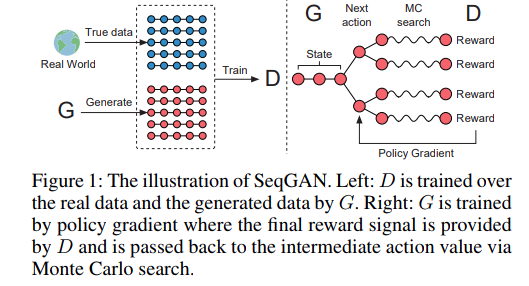
\includegraphics[width=10cm]{./img/seqgan.png}
\caption{SeqGAN Figure1 より引用}
\end{figure}

 それでは式を用いてガリガリと動きを示していきましょう。まずは Generator です。これは次のように示すことが出来ます。なお実装上はオリジナルの多分 LSTM を使っています。ここで \(s\) とは状態を表しており、つまりは生成された系列です。LSTM を用いて生成しているため、 \(y_t\) は確率の形で求められます。 SeqGAN ではここで multinomial 分布よりサンプリング (つまりその確率のところから良い感じに重み付けして1単語取ってくる) して次の単語 \(y_t\) を決定し、 \(s'=Y_{1:t}\) とします。ちなみに強化学習分野において \(s\) は状態、 \(a\) は行動と呼び、状態 \(s\) の時に 行動 \(a\) を取ることで次の状態 \(s'\) へ遷移する、と読むことが出来ます。
\begin{eqnarray}
G_{\theta} (a = y_t | s = Y_{1:t-1}) \ where\ y_i \in \mathcal{Y}\ \text{ is} \ \text{vocabulary}
\end{eqnarray}

 次に Discriminator です。繰り返しますが、Discriminator は、現実の文と生成された完全な文との真贋判定です。なので次のような式で表されます。注意として、Tは系列長ですが固定サイズです。例えば本来の文の長さが 9 であって T = 12 ならば文の後ろに padding が加えられます。(おそらくこのネットワークのために、本モデルは文長の分散にそこまで強くないです。まあ、本評価基準では長い文さえ生成できれば良いので、問題にはなりません。)

\begin{eqnarray}
D_{\phi} (s = Y_{1:T})
\end{eqnarray}

そしてここから方策勾配法について抉っていきます。以下は強化学習を多少知っている方でないとしんどいので頑張って下さい。まず強化学習の方策 \(J(\theta)\) を以下の式で表します。この方策勾配法は Generator を訓練するので、引数は \(\theta\) です。込み入っているので補足すると、期待値 \(\mathbb{E}\) を取っているところでは、「初期状態 \(s_0\) と \(\theta\) を与えられた時に、生成された文の報酬 \(R_T\) の期待値を最大化する」、と言っています。これはつまり Generator の y\textsubscript{1} を生成する確率 \(G_{\theta}(y_1|s_0)\) に、行動価値関数 \(Q\) をかけ合わせて周辺化 ( \(\mathcal{Y}\) の全ての単語で計算 ) したものと考えることが出来ます。

\begin{eqnarray}
J(\theta) = \mathbb{E}[R_T | s_0, \theta] = \sum_{y_1 \in \mathcal{Y}} G_{\theta}(y_1 | s_0) \cdot Q^{G_{\theta}}_{D_{\phi}}(s_0, y_1)
\end{eqnarray}

ここで行動価値関数へ与えられる状態+行動について考えてみます。仮に行動価値関数に与えられる状態が \(Y_{1:T-1}\) で 行動が \(y_T\) であったとき、生成される系列は \(Y_{1:T}\) だということがわかります。これは Discriminator に入れる値であるので、行動価値関数は、次のとおりです。

\begin{eqnarray}
Q^{G_{\theta}}_{D_{\phi}}(s = Y_{1:t-1}, y_t) = D_{\phi}(Y_{1:t}) \  \ \text{if} \ t = T
\end{eqnarray}

もし与えられる状態が \(Y_{1:T-1}\) でない場合、完全な系列ではないので Discriminator に入れることが出来ません。困った。\\
 そんなわけで仮にもし生成するんだとしたら、という \textbf{シミュレーション} を行います。使うのは モンテカルロサーチという手法です。
 まず なんかよくわからない Generator \(G_{\beta}\) を用意します (実装では \(G_{\theta}\) を使っています。パラメータも共有のようです)。\\
 次に \(G_{\beta}\) に状態 \(s = Y_{1:t}\) を入れて、シミュレーションによって系列長 \(T\) になるまでサンプルします。そしてこれを \(N\) 回行います。サンプルは \(G_{\beta}\) が出してくる \(y_{t+1}\) の確率値に基づく multinomial 分布に従って行われます。

\begin{eqnarray}
{Y_{1:T}^1, \dots ,  Y_{1:T}^{N}} = MC^{G_{\beta}}(Y_{1:t};N)
\end{eqnarray}

 シミュレーション結果が求まったので、それぞれの結果について Discriminator で報酬を求めます。この報酬の平均値を取れば、状態 \(s = Y_{1:t}\) が得られるであろう報酬を見積もることが出来ます。そしてこれが行動価値関数になるわけです。

\begin{eqnarray}
Q^{G_{\theta}}_{D_{\phi}}(s = Y_{1:t-1}, y_t) = \cfrac{1}{N}\sum^{N}_{n=1} D_{\phi}(Y^n_{1:T}),\ Y^n_{1:T} \in MC^{G_{\beta}}(Y_{1:t};N) \  \ \text{if} \ t < T
\end{eqnarray}

ここで出てくるのが強化学習で用いられる REINFORECE algorithm という手法です。 REINFORECE algorithm は 方策 \(J(\theta)\) を更新することで


\section{実装はどこ?再現実験したいんだけど}
\label{sec:orgbeb2989}
\href{https://github.com/LantaoYu/SeqGAN}{公式の実装} か、 \href{https://github.com/geek-ai/Texygen}{Texygen} を参考にすると良いと思います. 但し TF 1.x 系なのでそのうち書き直す必要があると思います (dockerize して TF 1.x の最新にアップデートしたものは \url{https://github.com/MokkeMeguru/Texygen} に持ってきています). とはいえ、 RNN の実装からオリジナルなので、TF 2.x で同じ実装が出来るかと言われるとかなり厳しいです.
\section{読んだ感想とか}
\label{sec:org278aa8c}
\section{付録: MLE (maximum likelihood estimation) って何?}
\label{sec:org3c2a9a0}
\end{document}
